\def\FigureWidth{492bp}
\def\FigureHeight{142bp}
% Common standalone PDF wrapper. Run latexmk from this directory.
\documentclass{article}
\usepackage[paperwidth=\FigureWidth,paperheight=\FigureHeight,margin=0pt]{geometry}
\usepackage[T1]{fontenc}
\usepackage{helvet}
\usepackage{tikz}
\usetikzlibrary{arrows.meta}
% Generated by scripts/export_report_figure_data.py; do not hand-edit.
% Dated figure inputs, not a second source of manuscript prose.
% site/data/benchmark-index.json SHA-256: b8d10892e25fe0fe63856f31e1645b41ee7d0f277fedaf308bd8f707852dbff2
% site/data/radar.json SHA-256: 83e33bd88be7639b2876e33c3c1fa18a1980b06ff721ee10cf8cf0d923bef703
\newcommand{\ReportDataCutoff}{2026-09-06}
\newcommand{\ReportObservationCount}{10702}
\newcommand{\ReportArtifactCount}{6304}
\newcommand{\ReportSnapshotCount}{45}
\newcommand{\ReportCatalogCount}{1283}
\newcommand{\ReportCatalogSourceCount}{4}
\newcommand{\ReportLLMStatsCount}{687}
\newcommand{\ReportOpenCompassCount}{461}
\newcommand{\ReportArtificialAnalysisCount}{25}
\newcommand{\ReportModelReportCount}{110}
\newcommand{\ReportSourceMaximum}{3394}
\newcommand{\ReportSourceBars}{%
  \SourceBar{0}{Hugging Face}{3394}%
  \SourceBar{1}{GitHub}{2423}%
  \SourceBar{2}{arXiv}{1899}%
  \SourceBar{3}{Semantic Scholar}{1039}%
  \SourceBar{4}{OpenAlex}{777}%
  \SourceBar{5}{8 other labels}{1170}%
}

\renewcommand{\familydefault}{\sfdefault}
\definecolor{RadarNavy}{HTML}{12233F}
\definecolor{RadarInk}{HTML}{243247}
\definecolor{RadarMuted}{HTML}{5C6B80}
\definecolor{RadarBlue}{HTML}{2563EB}
\definecolor{RadarSky}{HTML}{EAF1FF}
\definecolor{RadarTeal}{HTML}{0F766E}
\definecolor{RadarPaleTeal}{HTML}{E7F3F1}
\definecolor{RadarAmber}{HTML}{E99210}
\definecolor{RadarPaleAmber}{HTML}{FFF4DC}
\definecolor{RadarRule}{HTML}{D7DFEA}
\definecolor{RadarTrack}{HTML}{EFF3F8}
\definecolor{RadarPurple}{HTML}{7C3AED}
\definecolor{RadarCyan}{HTML}{14919B}
\definecolor{RadarGray}{HTML}{94A3B8}
\newcommand{\ReportNumber}[1]{\pgfmathprintnumber[fixed,precision=0,1000 sep={,},assume math mode=true]{#1}}
\pagestyle{empty}
\setlength{\parindent}{0pt}
\begin{document}
\null
\begin{tikzpicture}[remember picture,overlay,shift={(current page.south west)},
  x=1bp,y=1bp,every node/.style={inner sep=0pt,text=RadarInk,font=\sffamily\fontsize{8}{10}\selectfont}]

\draw[fill=RadarSky,draw=RadarBlue,line width=.6bp] (1,83) rectangle (491,141);
\foreach \x in {123,246,369} {\draw[white,line width=.6bp] (\x,83) -- (\x,141);}
\foreach \x/\value/\label in {
  62/\ReportObservationCount/{source observations\\across \ReportSnapshotCount{} snapshots},
  185/\ReportArtifactCount/{unique artifacts in the\\cumulative evidence graph},
  308/\ReportCatalogCount/{searchable benchmark\\records, including unscored},
  430/\ReportCatalogSourceCount/{catalog sources\\with source labels retained}} {
  \node[text=RadarNavy,font=\sffamily\bfseries\fontsize{21}{23}\selectfont] at (\x,123) {\ReportNumber{\value}};
  \node[align=center,text=RadarMuted,font=\sffamily\fontsize{7.6}{9.4}\selectfont] at (\x,98) {\label};
}
\draw[fill=RadarPaleAmber,draw=RadarAmber,line width=.6bp] (1,18) rectangle (491,69);
\node[anchor=west,text width=466bp,text=RadarNavy,font=\sffamily\bfseries\fontsize{10}{13}\selectfont] at (13,44)
  {Benchmark Radar brings daily discoveries, catalog search, model-report adoption, and sourced scores into one place. Each count measures a different kind of evidence.};
\node[text=RadarMuted,font=\sffamily\itshape\fontsize{7}{9}\selectfont] at (246,7)
  {Data cutoff: \ReportDataCutoff. Catalog records and discovery observations are separate units.};
\end{tikzpicture}
\end{document}
